\documentclass[aspectratio=169]{beamer}
\usetheme{Madrid}
\usecolortheme{crane}

\usepackage[utf8]{inputenc}
\usepackage[T1]{fontenc}
\usepackage{graphicx}
\usepackage{tikz}
\usepackage{listings}

\definecolor{primary}{RGB}{220, 38, 38}
\definecolor{secondary}{RGB}{248, 113, 113}
\definecolor{dark}{RGB}{30, 30, 46}

\setbeamercolor{palette primary}{bg=primary,fg=white}
\setbeamercolor{palette secondary}{bg=secondary,fg=white}
\setbeamercolor{structure}{fg=primary}
\setbeamercolor{title}{fg=primary}

\lstset{
    basicstyle=\ttfamily\small,
    breaklines=true
}

\title[Project Presentation]{[Your Project Name]}
\subtitle{Final Project Presentation}
\author{[Team Member 1, Team Member 2, Team Member 3]}
\institute{State University of Zanzibar (SUZA)\\BSc Computer Science}
\date{[Presentation Date]}

\begin{document}

% Title Slide
\begin{frame}
    \titlepage
\end{frame}

% Table of Contents
\begin{frame}{Outline}
    \tableofcontents
\end{frame}

% Section 1: Introduction
\section{Introduction}

\begin{frame}{Project Overview}
    \begin{block}{Project Name}
        [Your Project Name]
    \end{block}

    \begin{block}{Problem Statement}
        \begin{itemize}
            \item What problem are you solving?
            \item Why is this problem important?
            \item Who faces this problem?
        \end{itemize}
    \end{block}
\end{frame}

\begin{frame}{Objectives}
    \begin{enumerate}
        \item \textbf{Primary Objective:} [Main goal of the project]
        \item \textbf{Secondary Objectives:}
        \begin{itemize}
            \item [Objective 2]
            \item [Objective 3]
            \item [Objective 4]
        \end{itemize}
    \end{enumerate}
\end{frame}

\begin{frame}{Target Users}
    \begin{columns}
        \column{0.5\textwidth}
        \textbf{Primary Users:}
        \begin{itemize}
            \item [User type 1]
            \item [User type 2]
        \end{itemize}

        \column{0.5\textwidth}
        \textbf{User Needs:}
        \begin{itemize}
            \item [Need 1]
            \item [Need 2]
            \item [Need 3]
        \end{itemize}
    \end{columns}
\end{frame}

% Section 2: Solution
\section{Solution}

\begin{frame}{Proposed Solution}
    \begin{block}{How We Solved It}
        [Brief description of your solution - 2-3 sentences]
    \end{block}

    \textbf{Key Features:}
    \begin{enumerate}
        \item [Feature 1]
        \item [Feature 2]
        \item [Feature 3]
        \item [Feature 4]
    \end{enumerate}
\end{frame}

\begin{frame}{System Architecture}
    \begin{center}
        % Replace with your actual architecture diagram
        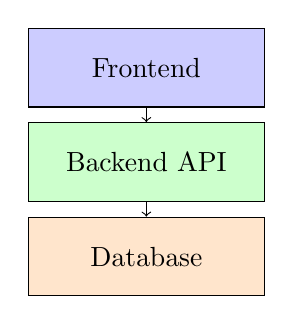
\begin{tikzpicture}[scale=0.8]
            \node[draw, rectangle, minimum width=3cm, minimum height=1cm, fill=blue!20] (client) at (0,3) {Frontend};
            \node[draw, rectangle, minimum width=3cm, minimum height=1cm, fill=green!20] (server) at (0,1.5) {Backend API};
            \node[draw, rectangle, minimum width=3cm, minimum height=1cm, fill=orange!20] (db) at (0,0) {Database};

            \draw[->] (client) -- (server);
            \draw[->] (server) -- (db);
        \end{tikzpicture}
    \end{center}

    \begin{itemize}
        \item \textbf{Frontend:} [Technology used]
        \item \textbf{Backend:} [Technology used]
        \item \textbf{Database:} [Technology used]
    \end{itemize}
\end{frame}

\begin{frame}{Technology Stack}
    \begin{columns}
        \column{0.5\textwidth}
        \textbf{Frontend:}
        \begin{itemize}
            \item [Framework/Library]
            \item [CSS Framework]
            \item [Other tools]
        \end{itemize}

        \textbf{Backend:}
        \begin{itemize}
            \item [Language/Framework]
            \item [Authentication]
            \item [Other tools]
        \end{itemize}

        \column{0.5\textwidth}
        \textbf{Database:}
        \begin{itemize}
            \item [Database type]
        \end{itemize}

        \textbf{DevOps:}
        \begin{itemize}
            \item Git/GitHub
            \item [Hosting platform]
            \item [CI/CD if used]
        \end{itemize}
    \end{columns}
\end{frame}

% Section 3: Demo
\section{Demo}

\begin{frame}{Live Demo}
    \begin{center}
        \Huge Demo Time!
    \end{center}

    \textbf{Demo Flow:}
    \begin{enumerate}
        \item User Registration/Login
        \item [Main Feature 1]
        \item [Main Feature 2]
        \item [Main Feature 3]
    \end{enumerate}

    \vspace{0.5cm}
    \small URL: [Your deployed application URL]
\end{frame}

\begin{frame}{Screenshots}
    \begin{columns}
        \column{0.5\textwidth}
        \begin{block}{Home Page}
            [Insert screenshot or describe]
        \end{block}

        \column{0.5\textwidth}
        \begin{block}{Main Feature}
            [Insert screenshot or describe]
        \end{block}
    \end{columns}
\end{frame}

% Section 4: Development Process
\section{Development Process}

\begin{frame}{Methodology}
    \textbf{Agile/Scrum Approach:}
    \begin{itemize}
        \item Sprint Duration: [X weeks]
        \item Total Sprints: [Number]
        \item Tools Used: [Trello/GitHub Projects/Jira]
    \end{itemize}

    \vspace{0.5cm}
    \textbf{Sprint Breakdown:}
    \begin{enumerate}
        \item Sprint 1: [Focus area]
        \item Sprint 2: [Focus area]
        \item Sprint 3: [Focus area]
    \end{enumerate}
\end{frame}

\begin{frame}{Team Roles}
    \begin{tabular}{|l|l|l|}
        \hline
        \textbf{Name} & \textbf{Role} & \textbf{Responsibilities} \\
        \hline
        [Name 1] & Team Lead & [Responsibilities] \\
        \hline
        [Name 2] & Frontend Dev & [Responsibilities] \\
        \hline
        [Name 3] & Backend Dev & [Responsibilities] \\
        \hline
    \end{tabular}
\end{frame}

\begin{frame}{Git Statistics}
    \begin{columns}
        \column{0.5\textwidth}
        \begin{itemize}
            \item Total Commits: [Number]
            \item Pull Requests: [Number]
            \item Branches: [Number]
        \end{itemize}

        \column{0.5\textwidth}
        \textbf{Contribution:}
        \begin{itemize}
            \item [Member 1]: [X commits]
            \item [Member 2]: [X commits]
            \item [Member 3]: [X commits]
        \end{itemize}
    \end{columns}

    \vspace{0.5cm}
    Repository: \url{https://github.com/[username]/[repo]}
\end{frame}

% Section 5: Testing
\section{Testing}

\begin{frame}{Testing Summary}
    \begin{block}{Test Coverage}
        \begin{itemize}
            \item Unit Tests: [Number] tests
            \item Integration Tests: [Number] tests
            \item Test Pass Rate: [Percentage]\%
        \end{itemize}
    \end{block}

    \begin{block}{Key Test Areas}
        \begin{itemize}
            \item Authentication
            \item [Feature 1]
            \item [Feature 2]
            \item API Endpoints
        \end{itemize}
    \end{block}
\end{frame}

% Section 6: Challenges
\section{Challenges \& Lessons}

\begin{frame}{Challenges Faced}
    \begin{enumerate}
        \item \textbf{Challenge 1:} [Description]
        \begin{itemize}
            \item Solution: [How you solved it]
        \end{itemize}

        \item \textbf{Challenge 2:} [Description]
        \begin{itemize}
            \item Solution: [How you solved it]
        \end{itemize}

        \item \textbf{Challenge 3:} [Description]
        \begin{itemize}
            \item Solution: [How you solved it]
        \end{itemize}
    \end{enumerate}
\end{frame}

\begin{frame}{Lessons Learned}
    \begin{itemize}
        \item \textbf{Technical:} [What you learned technically]
        \item \textbf{Teamwork:} [What you learned about collaboration]
        \item \textbf{Project Management:} [What you learned about managing projects]
        \item \textbf{Communication:} [What you learned about communication]
    \end{itemize}
\end{frame}

% Section 7: Future Work
\section{Future Work}

\begin{frame}{Future Improvements}
    \textbf{Short-term (Next Sprint):}
    \begin{itemize}
        \item [Improvement 1]
        \item [Improvement 2]
    \end{itemize}

    \textbf{Long-term:}
    \begin{itemize}
        \item [Feature addition 1]
        \item [Feature addition 2]
        \item [Scalability improvements]
    \end{itemize}
\end{frame}

% Section 8: Conclusion
\section{Conclusion}

\begin{frame}{Summary}
    \begin{block}{What We Built}
        [One sentence summary of your project]
    \end{block}

    \begin{block}{Key Achievements}
        \begin{itemize}
            \item [Achievement 1]
            \item [Achievement 2]
            \item [Achievement 3]
        \end{itemize}
    \end{block}

    \begin{block}{Impact}
        [How this project can help users]
    \end{block}
\end{frame}

\begin{frame}{Thank You!}
    \begin{center}
        \Huge Questions?
    \end{center}

    \vspace{1cm}
    \textbf{Contact:}
    \begin{itemize}
        \item Repository: \url{https://github.com/[username]/[repo]}
        \item Demo: \url{[Your deployed URL]}
        \item Email: [team email]
    \end{itemize}
\end{frame}

\end{document}
